\section{Durchführung und Versuchsaufbau}
\label{sec:Durchführung}

\subsection{Versuchsaufbau}
Wie in \autoref{sec:Theorie} beschrieben, wird monochromatisches Licht benötigt, um den Photoeffekt herbeizuführen. Da in diesem Versuch die Elektronenenergie in Abhängigkeit 
der Wellenlänge des Lichtes untersucht werden soll, wird eine Hg-Spektrallampe verwendet. Diese emittiert einen Großteil des sichtbaren Spektrums.
Um nun monochromatisches Licht zu erhalten wird der optische Aufbau aus \autoref{fig:versuchsaufbau} verwendet. 

\begin{figure}[H]
    \centering
    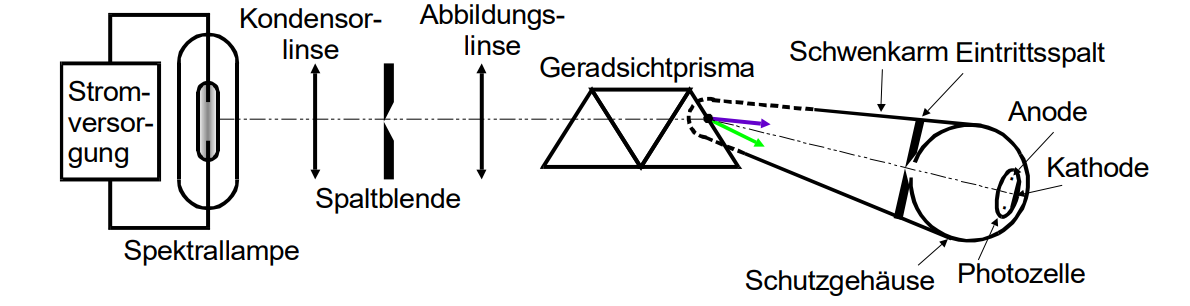
\includegraphics[width=1\textwidth, height = 5cm]{img/versuchsaufbau.png}
    \caption{Optischer Aufbau \cite{V500}.}
    \label{fig:versuchsaufbau}
\end{figure}

Das von der Hg-Lampe erzeugte Licht wird von der Kondensorlinse gebündelt und läuft dann durch die Spaltblende. Dann wird das Licht von der Abbildungslinse auf das 
Geradsichtprisma gebündelt, welcher das Licht in einzelne Wellenlängen aufspaltet. Je nach gewünschter Wellenlänge kann mit einem Schwenkarm das monochromatische Licht
auf die Photozelle gerichtet werden. 
Die wichtigsten Linien des Hg-Spektrums sind in \autoref{tab:hg-spektrum} aufgelistet.

\begin{table}[H]
    \centering
    \caption{Wichtige Linien des Hg-Spektrums.}
    \begin{tabular}{c c c}
        \toprule
        $\lambda \,[\unit{nm}]$ & Farbe & Intensität\\
        \midrule
        577, 579 & gelb & stark\\
        546 & grün & stark\\
        492 & blaugrün & gering\\
        434, 435, 436 & violett & stark\\
        (408), 405 & violett & (gering), stark\\
        365, 366 & ultraviolett & stark\\
        \bottomrule
    \end{tabular}
    \label{tab:hg-spektrum}
\end{table}

Für die Gegenfeldmethode wird ein Voltmeter angeschlossen mit dem verschiedene Potentiale an die Photozelle angelegt werden können. Mit dem verwendeten Gerät kann ein Bereich von
$\pm \SI{2}{V}$ oder $\pm \SI{20}{V}$ angelegt werden.\\
Um den Photostrom messen zu können wird ein Picoamperemeter angeschlossen. Da die Ströme sehr klein sind und so auch sensibel für Störungen, sollte ein Koaxialkabel zur Verbindung
der einzelnen Elemente benutzt werden. In \autoref{fig:schaltbild} ist der Schaltkreis gezeigt. In \autoref{fig:real} ist ein Foto des Aufbaus zu sehen.
\begin{figure}[H]
    \centering
    \begin{subfigure}[b]{0.49\textwidth}
        \centering
        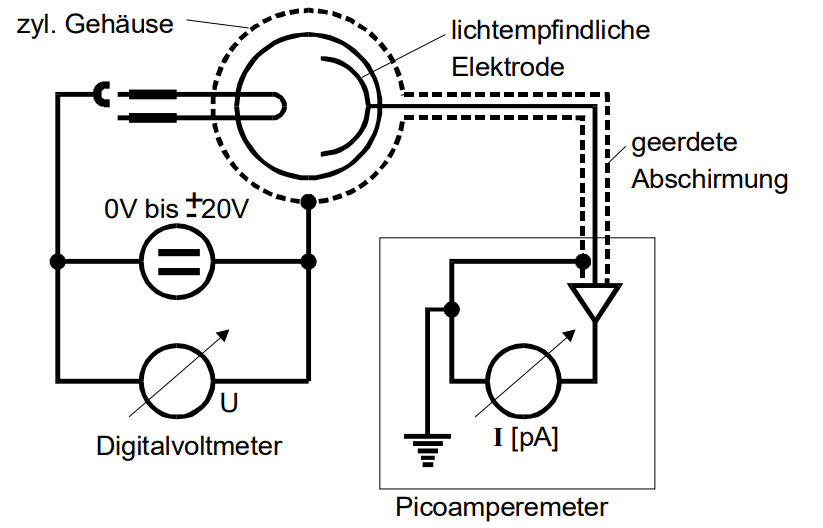
\includegraphics[width=7.5cm, height=5.5cm]{img/schaltbild.png}
        \caption[]
        {{\small Schaltbild.}}    
        \label{fig:schaltbild}
    \end{subfigure}
    \hfill
    \begin{subfigure}[b]{0.49\textwidth}  
        \centering 
        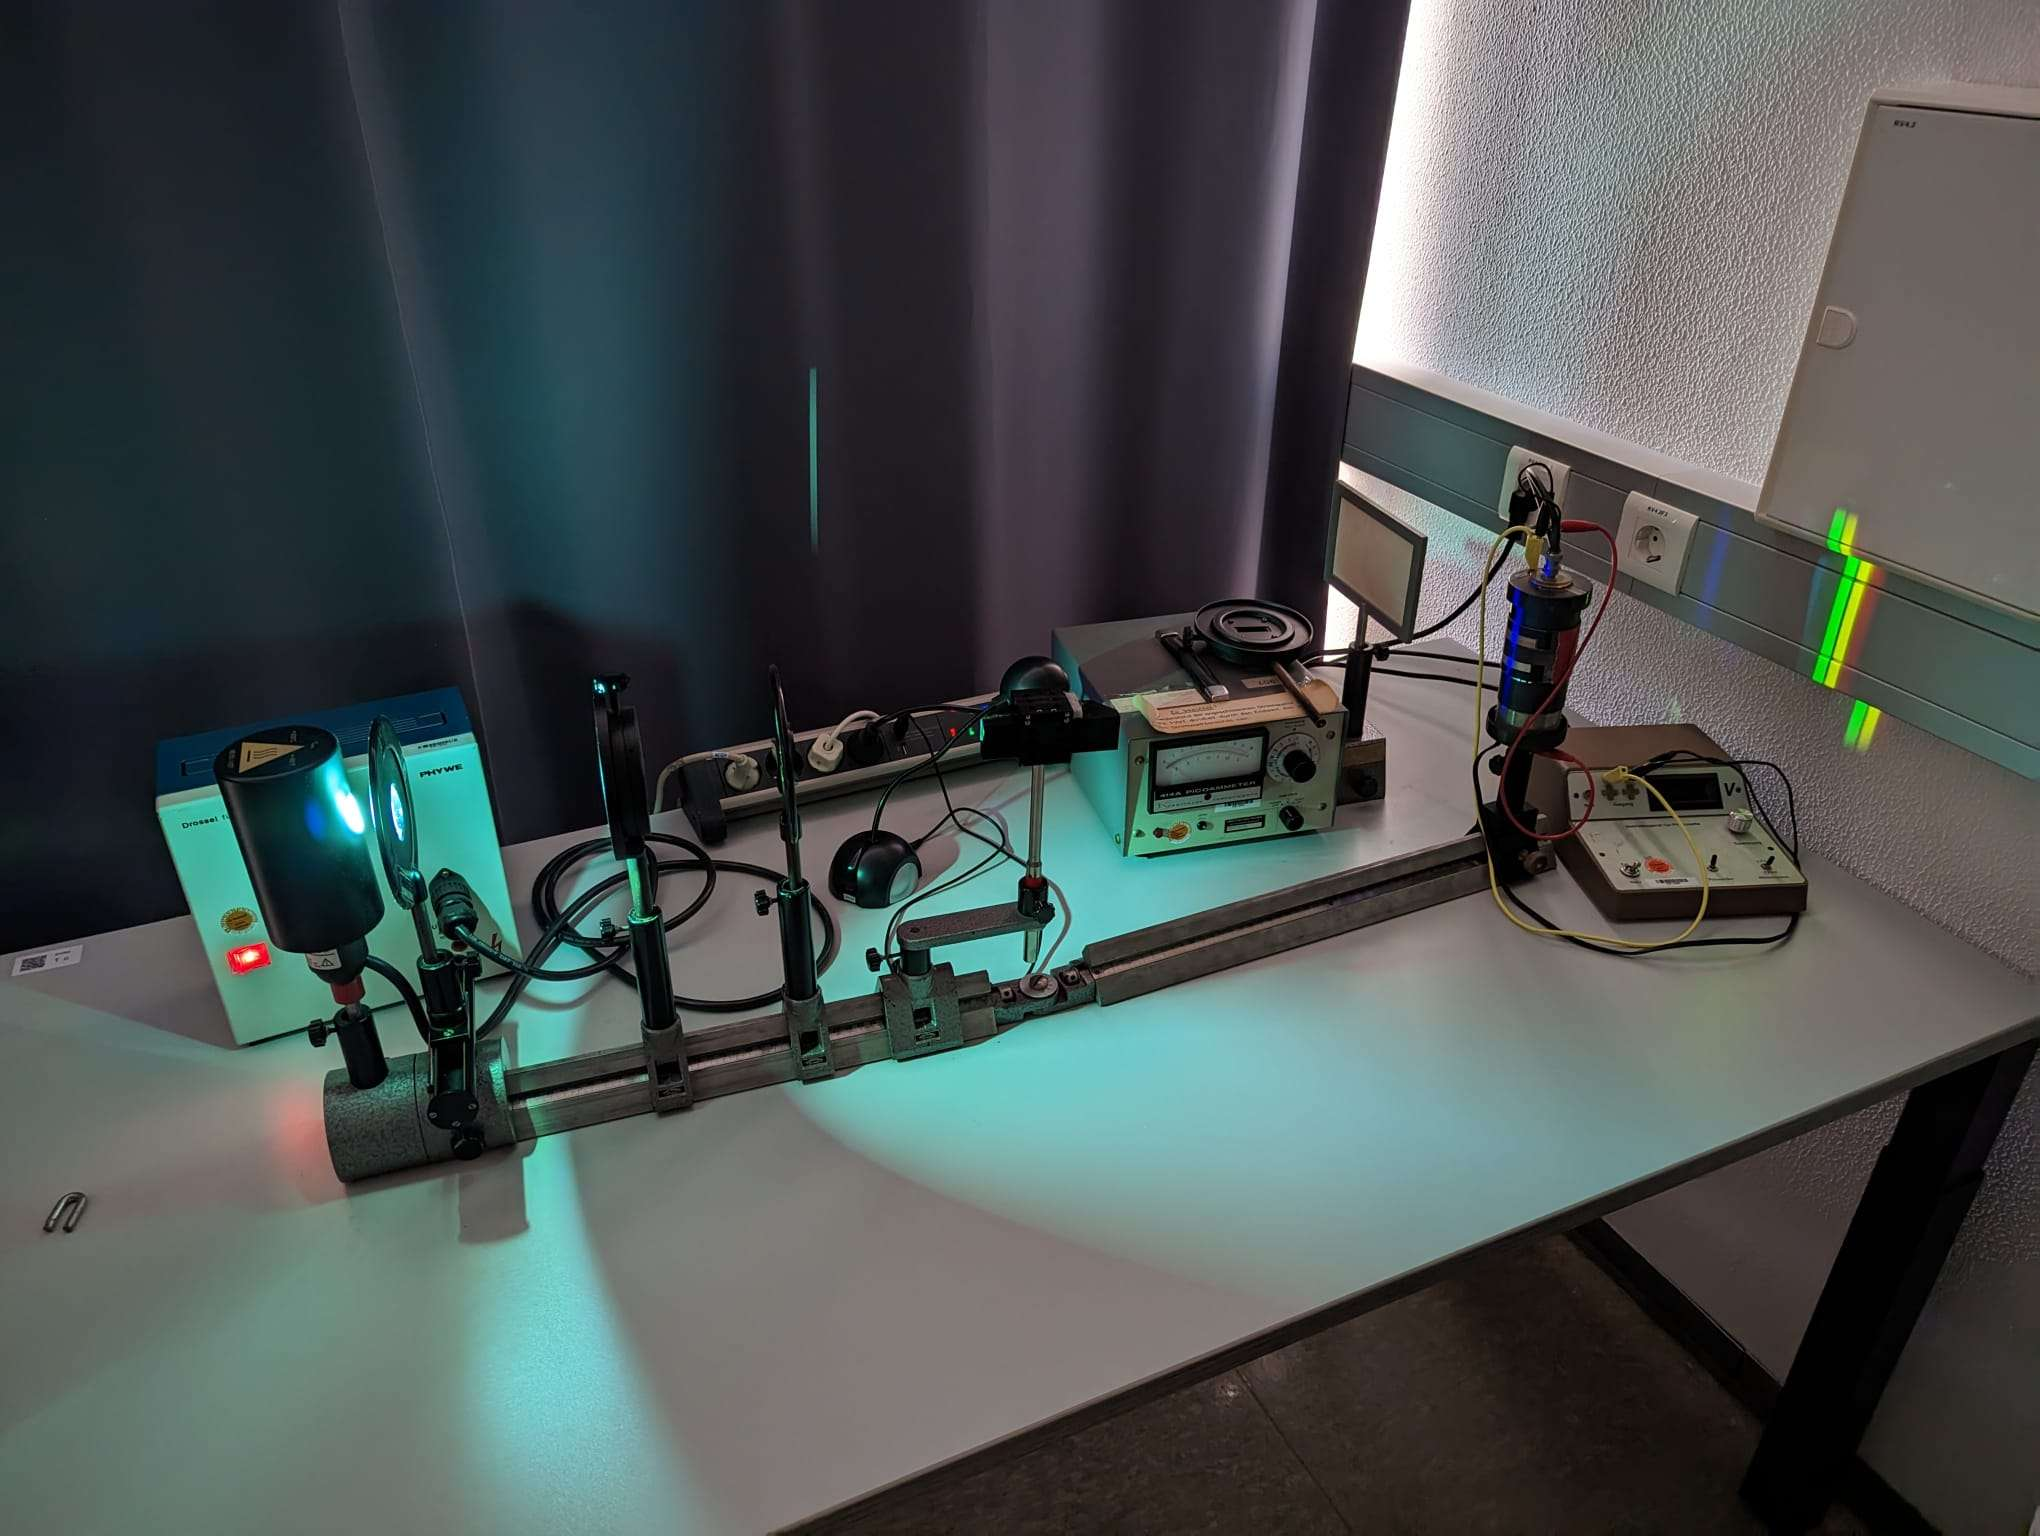
\includegraphics[width=7.5cm, height=6.5cm]{img/aufbau_real.jpg}
        \caption[]
        {{\small Foto des Aufbaus.}}    
        \label{fig:real}
    \end{subfigure}
\end{figure}

\subsection{Durchführung}
Es werden vier verschiedene Wellenlängen untersucht. Für gelb $\lambda_{gelb} \approx \SI{578}{nm}$ wird der Photostrom in $\SI{0.5}{V}$ Schritten auf einem Spannungsintervall
von $\SI{-20}{V}$ bis $\SI{20}{V}$ gemessen. Für rot $\lambda_{rot} \approx \SI{650}{nm}$, lila $\lambda_{violett} \approx \SI{435}{nm}$ und grün $\lambda_{gruen} \approx \SI{546}{nm}$
wird in $\SI{0.1}{V}$ bis $\SI{0.05}{V}$ Schritten auf einem Spannungsintervall von $\SI{-2}{V}$ bis $\SI{2}{V}$ gemessen.